% !TeX root = ./DLVCQuestions.tex
%
\section{Image classification}
\subsection{What is the task definition of image classification?}
Predict the label (picked from a set of possible labels) of an image, i.e.: what is visible on the image. Output could also be a distribution over labels to indicate confidence in result.

\subsection{Explain at least 5 challenges and give examples.}
\begin{itemize}
\item Viewpoint variation: A single instance of an object can be oriented in many ways with respect to the camera.
\item Scale variation: Visual classes often exhibit variation in their size (size in the real world, not only in terms of their extent in the image).
\item Deformation: Many objects of interest are not rigid bodies and can be deformed in extreme ways, e.g. water
\item Occlusion: Only a small portion of an object (as little as few pixels) could be visible.
\item Illumination conditions: The effects of illumination are drastic on the pixel level.
\item Background clutter: The objects of interest may blend into their environment, making them hard to identify.
\item Intra-class variation: The classes of interest can often be relatively broad, such as chair. There are many different types of these objects, each with their own appearance.
\item Abstraction (human able to recognize some doodle as the correct object usually---difficult to recognize for machines as e.g. difference between cow and dog in a doodle may be the presence of grass
\item Invariants (an object may be the same object if it's rotated by some degree. Other objects (e.g. ``6'' and ``9'') are not invariant under rotation
\end{itemize}

\subsection{What is object detection and how does it differ from classification?}
Object detection tries to find all objects present in an image whereas in image classification a label is assigned to the whole image. Object detection can be reduced to image classification (classify various parts of the image and combine results)

%
\section{Datasets}
\subsection{Why do we need datasets?}
Data required for training and testing of model. 
\subsection{What are the challenges of dataset collection and annotation in deep learning?}Datasets should be sampled from the same distribution as images which are then classified, i.e. it should span the whole space of possible features associated with each class. For example if dataset contains only cats run over by car a model trained with this set will have difficulties recognizing healthy cats.
\subsection{Explain the purpose of the different subsets.}
\begin{itemize}
\item Training set: Used to train the model
\item Validation set: Used to train hyperparameters
\item Test set: Final performance analysis. 
\end{itemize}
Model is trained with training set and then evaluated with validation set. Then some other hyperparameters are chosen (e.g. lower learning rate, \ldots) and the step is repeated until there is no further improvement to the model. The datasets have to be disjunct as else it would be ``learning to the test'' (e.g. model is a hashmap containing the hash of the image and the correct class. Would work if testset is contained in training set but completely useless for new data)

\subsection{What is the rule of thumb about how many images per classes are needed for CNNs to perform well?}
At least 5000 per class---more is better though.
%
\section{Case study}
\begin{quote}
Assume a company asks you to develop an application that is able to predict which kind of bird is depicted in a given image. List and explain the individual steps you’d follow to solve this problem using deep learning.
\end{quote}
\begin{enumerate}
\item (Set up some machine that allows to train the model with hardware acceleration)
\item Ask what kind of birds should be distinguished from each other (e.g. is ``parrot'' enough or should it be ``macaw parrot'' or even ``Ara'' or ``Military macaw'')
\item Only sitting birds or also while they're flying? 
\item Look for dataset that fulfills the conditions resulting from the above questions
\item Proceed in the usual order to train a model:
\begin{itemize}
\item Set up training process
\item Find suitable NN architecture
\item Augment dataset 
\item Find hyperparameters and tune them until accuracy is good enough
\end{itemize}
\end{enumerate}
%
\section{DL Motivation}
\subsection{What is the motivation for solving vision tasks via machine learning?}
\begin{minipage}{0.6\textwidth}
\begin{itemize}
\item Rule based system: handwritten AI where an expert implements all rules (decision boundaries)
\item Classic machine learning: The features are designed and the algorithm then maps the features to the boundaries
\item Representation learning: The features are trained on the data and mapped to output.
\item Deep learning: There are low and high level features and the algorithm learns how to train the features, how to combine them to higher level features and how to map the to the output
\end{itemize}
\end{minipage}
\begin{minipage}{0.4\textwidth}\hspace{0.25cm}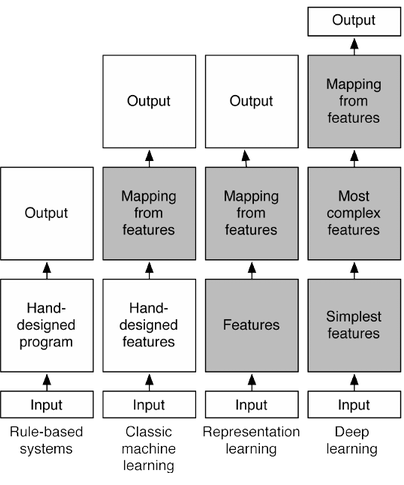
\includegraphics[width=1.25\textwidth]{./img/motivation.png}
\end{minipage}
\subsection{What is a machine learning algorithm and how are they used for solving image classification problems?}
A machine learning algorithm is a method of statistical analysis that automates analytical model building. Their aim is to find hidden insights without being programmed where to look. 
This is applied for image classification by providing a dataset of labelled images which are then used to extract features which are used to infer the class of an image. 

Applying rule based systems would be completely overwhelming (e.g. if there are 45\% blue pixels and 55\% white pixels it's a boat \ldots)
%
\section{Classification \& regression, un-/supervised learning}
\subsection{Explain the differences between classification and regression and supervised vs. unsupervised learning}
Classification is used to predict discrete outputs (e.g. an animal is a dog or a cat but not some 50:50 mixture of both) whereas regression is used to predict continuous values (e.g. IQ, height, time \ldots).

Supervised learning uses a training dataset where the desired prediction is already known and the algorithm tries to find a model that would come to the same conclusions. 

Unsupervised learning only uses a dataset and the algorithm tries to find some structure in it (e.g. SOMs, EM-algorithm, PCA)
\subsection{What do discriminative and generative models learn }
Discriminative models learn the boundary between classes $P(y|x)$ (estimate response $y$ when given input $x$ whereas generative models learn the underlying distribution $P(x,y)$.

SVN and NN are discriminative, Naive Bayes and Hidden Markov models are generative.
\subsection{How can generative models be used for classification?}
It uses the distribution $P(x,y)$ to estimate which response $y$ is most likely to cause the given input $x$ ($\text{argmax}_y P(x|y)P(y)$). Though generative models can be used for classification discriminative models usually perform better. 
%
\section{Testdata}
\subsection{Why are machine learning algorithms tested on data unseen during training?}
The goal is to have a model that can predict new data. Therefore it's a good idea to measure exactly this as quality criterion by using unseen data for testing purposes. The same applies to the validation data---optimize the model to perform well on data not seen during training. If this would not be done model after training would be completely overfitted and would perform well on the training data (which is useless) but not necessarily well or even good on new data.
\subsection{How can such algorithms perform well on unseen data?}
If the model is not overfitted it should recognize general features (``wheels in the lower left corner'') of the sample but not very specific features (e.g.: hash of the image). 
\subsection{What does dataset bias mean? }
When a model was trained on a dataset the model will usually be applied to new problems (samples not yet found in the dataset). As the model will only take into consideration information from the training set this dataset should be sampled without bias from the same distribution as the samples that are then used in production. If this is not the case the model won't perform well. For example a model trained on whales and bees will have difficulties to predict whether a cow is an insect or a mammal.
%
\section{Performance measures}
\subsection{How is the performance of a classifier measured?}
For classification the accuracy is used to measure the performance. The predictions are compared with the target labels and the accuracy is defined as the fraction of correctly classified samples (the error rate is the complement of this).
\subsection{Which factors determine the performance, and how is underfitting and overfitting related to these factors?}
The performance of an algorithm is determined by two factors
\begin{itemize}
\item Ability to minimize training error (if this fails: underfitting)
\item Ability to minimize gap between training and test error (if the first succeeds but this fails: overfitting)
\end{itemize}
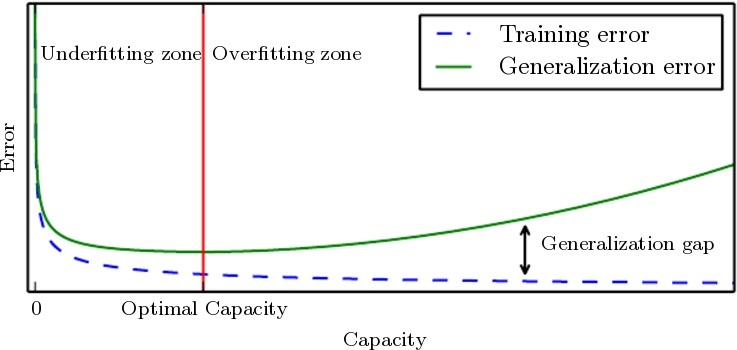
\includegraphics[width=\textwidth]{./img/overfit.png}
From left to right: underfit (low capacity), good model, overfit (high capacity)
%
\section{Capacity, bias, variance}
\todo{Improve rather weak capacity answers}
\subsection{Explain the terms algorithm capacity, bias, and variance.}
\begin{itemize}
\item Algorithm capacity: the capacity is the ability to compute complex decision boundaries. If two models have the same validation error the model with lower capacity is usually preferred (``most parsimonious model'', AIC and BIC are formalizations of this notion in the context of linear regression)
\item Bias: If the capacity is too low the model struggles to fit the training set. This results in a high bias. 
\item Variance: If the capacity is too high the model fits the data too well which results in high variance and bigger generalization error
\end{itemize}
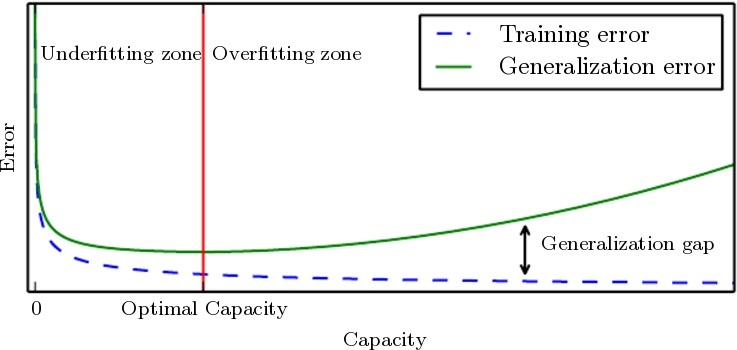
\includegraphics[width=\textwidth]{./img/capacity.jpeg}
When the capacity is too low neither the training error nor the test error can be reduced to the optimal point. The capacity is optimal when the test error is minimal. Starting from this point increasing the capacity may result in a lower training error due to overfitting but the test error increases again. The gap between training and test error is called generalization gap that results from tailoring the model too strongly to the training/validation data.
\subsection{Why does the training set size affect the optimal capacity of a model?}
When more training data is available the performance of the model will increase as the data reflects the problem better. This also results in a higher optimal performance
%
\section{Hyperparameter}
\subsection{What is a hyperparameter?}
In ML we try to find parameters for a model from datasets. This learning process may have its own parameters, these are called hyperparameters. They govern behaviour of the model learning, .e.g. the capacity of the resulting model.
\subsection{Name at least 3 hyperparameters in the context of deep learning using convolutional neural networks.}
\todo{maybe explain what these hyperparameters do}
\begin{enumerate}
\item Initial learning rate
\item Learning rate decay
\item Regularization strength
\item Momentum settings
\end{enumerate}
\subsection{What is the purpose of hyperparameter selection, which search strategies exist, and how do they work?}
Purpose is finding optimal settings to train the model. Gridsearch and random search are two common approaches, random search is usually preferred as one parameter may be insignificant for the result and much time would be wasted optimizing this parameter whereas with random search all HP spaces are explored independently. See picture below.

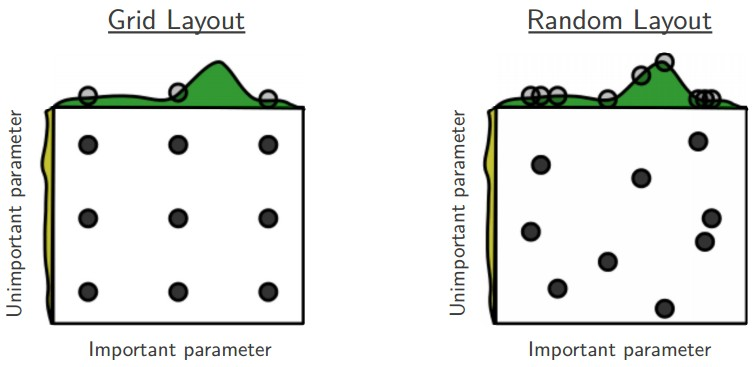
\includegraphics[width=\textwidth]{./img/gridsearchbad.jpeg}
%
\section{kNN}
\subsection{How does the k nearest neighbor classifier work?}
Find the k samples in the training set that are most similar to the current sample according to some similarity measure

\begin{itemize}
\item Training
\begin{itemize}
\item Preprocess data 
\item Transform images to vectors ($32\times 32\times 3 \text{ image }\to 32\cdot 32\cdot 3 = 3072$D vector) or use extracted feature vector
\item Split into training and validation data and optimize the hyperparameters (distance measure and $k$)
\end{itemize}
\item Classification
\begin{itemize}
\item Apply the same preprocessing  transformations as before
\item Find the k images that are most similar and use the most common label as prediction (or output the distribution of labels)
\end{itemize}
\end{itemize}

\subsection{Sketch of kNN}
\begin{minipage}{0.65\textwidth}
{Create a sketch for illustration, assuming a two-dimensional feature space and two different classes, Draw at least three training samples per class (must not lie on a line) as well as (roughly) the resulting decision boundaries.}

Image on right is kNN with two classes and $k=1$.
\end{minipage}
\begin{minipage}{0.4\textwidth}

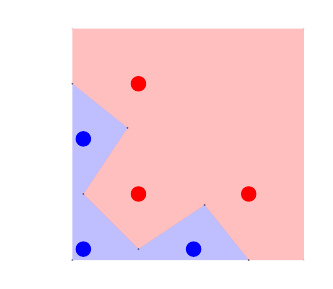
\begin{tikzpicture}[scale=1.4]
\draw[white] (-0.5,-0.1) rectangle(2,2);
\fill[blue] (0,0)circle(2pt);
\fill[blue] (1,0)circle(2pt);
\fill[blue] (0,1)circle(2pt);
\fill[red] (0.5,0.5)circle(2pt);
\fill[red] (1.5,0.5)circle(2pt);
\fill[red] (0.5,1.5)circle(2pt);
\def\pointset{(-0.1,1.5),(0.4,1.1),(0,0.5),(0.5,0),(1.1,0.4),(1.5,-0.1),(2,-0.1),(2,2),(-0.1,2)}
\foreach \x[count=\i] in \pointset
  \fill [opacity=0.1] \x circle(0.25pt) coordinate (mark-\i);
\fill [opacity=0.25,red]
  (mark-1) \foreach \x[count=\i] in \pointset{ -- (mark-\i) } -- cycle;

\def\pointset{(-0.1,1.5),(0.4,1.1),(0,0.5),(0.5,0),(1.1,0.4),(1.5,-0.1),(-0.1,-0.1)}
\foreach \x[count=\i] in \pointset
  \fill [opacity=0.5] \x circle(0.25pt) coordinate (mark-\i);
\fill [opacity=0.25,blue]
  (mark-1) \foreach \x[count=\i] in \pointset{ -- (mark-\i) } -- cycle;
\end{tikzpicture}
\end{minipage}
\subsection{What are the limitations of this classifier?}
\begin{itemize}
\item Classification performance is rather bad as sample has to be compared to all/most of the samples in the training set (can be improved with KDTree from $O(n)$ to $O(log(n)^d)$ or similar)
\item Does not recognize higher order features, e.g. ``presence of wheels'' but only uses similarity of features (pixels). Completely thrown off the track by e.g. different lighting or position of object in image (e.g. off center in sample and only centered pictures in training set)
\item Very sensitive to background
\end{itemize}
%
\section{Image Classification}
\subsection{Why do general machine learning algorithms (those expecting vector input) perform poorly on images?}
Images have spatial information, i.e. a pixel is correlated with the pixels in its surrounding. This additional information is not leveraged with general ML algorithms and thus the resulting performance is subpar.
\subsection{What is a feature, and what is the purpose of feature extraction?}
Features are used to classify something. If it has four wheels and 5 people can sit in it it is most likely a car. If it has four legs it's most likely not a human etc.

Feature extraction is used to get the features of a sample, e.g. are there eyes on the image, is the object curved, \ldots. These extracted features can then be used to classify an image.
\subsection{Explain the terms low-level feature and high-level feature.}
A low level feature would be the existence of edges in a certain direction or some color gradient. A high level feature is then built from a set of low level features, e.g. a face consists of a certain arrangment of strokes (the outline and nose and mouth) and round objects (eyes). An even higher level feature would then be a person consisting of various features such as ``face'', ``body'' and ``limbs''. 
%
\section{Parametric model}
\subsection{What is the definition of a parametric model?}
A model is a function that maps from the input space to the output space: $f:\mathbb R^D \to \mathbb R^T$. A parametric model also takes a finite vector of parameters $\theta$ to get from input $x$ to output $y$: $f(x,\theta) = y$.

Whereas the model for a kNN classifier (a non-parametric model) gets more complex the bigger the training set is a parametric model only has parameters that are better chosen if the training set gets larger. 
\subsection{What do the parameters of such models control (what effect do they have?), and how are they set?}
The parameters are determined by training the model with a trainingset which can be discarded afterwards. In a linear model the weight matrix and bias vector are the parameters and they govern the decision boundary $Wx + b$. 
%
\section{Linear model}
\subsection{What is a linear model, which types of parameters does it have, and what do they specify?}
A linear model tries to seperate the samples with linear functions. The samples are in a $D$-dimensional space and there are $T$ classes. The model then consists of $T$ decision boundaries of the form $y_t = \sum_i^D W_{ti} x_i + b_t$ or in short $y = Wx + b$. The weight matrix $W$ and the bias vector $b$ are the parameters. The resulting model is a set of decision boundaries where each boundary provides a value for each class. Usually the class with the highest score is then chosen as prediction. 

\begin{minipage}{0.32\textwidth}
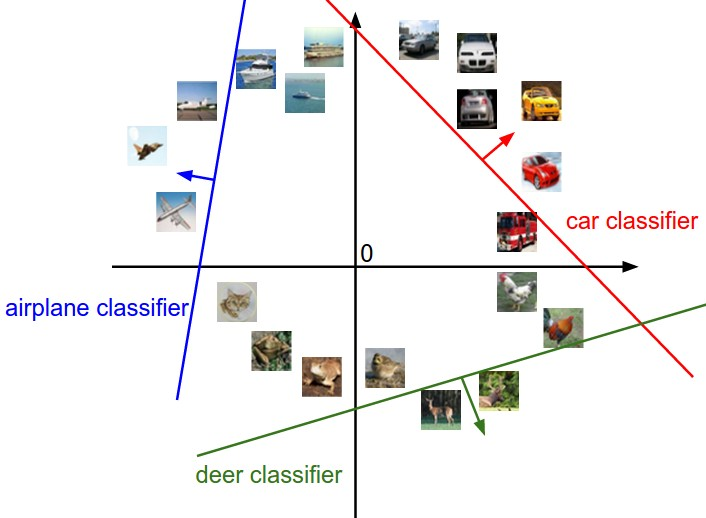
\includegraphics[width=0.95\textwidth]{./img/lclass.jpeg}
\end{minipage}\begin{minipage}{0.7\textwidth}
The output value of $f(x, \theta)$ has a score for each class where a positive number corresponds to the sample being on the side indicated with an arrow, meaning, that the sample is more likely than not a member of this class. The class with the highest score is then chosen as prediction. 
\end{minipage}
%
\section{Loss function}
\subsection{What is the purpose of a loss function?}
When training a parametric model an optimization algorithm the minimizes a loss function is used. The loss function has the parameters as input and the global minimum of $L(\theta)$ corresponds to the parameter setting that is optimal for the task at hand (classifying images).
\subsection{What does the cross-entropy loss on a dataset D measure?}
For classification usually cross-entropy loss used. CEL measures the dissimilarity of the real distribution from the predicted distribution. $H(p,q) = -\sum_x p(x) \ln q(x)$. $p,q$ are discrete probability distributions $p(x)\leq 0, \sum_x p(x) = 1$. The CEL of a dataset is then the sum of the CEL of all samples divided by the size of the dataset. 
\subsection{Which criteria must the ground-truth labels and predicted class-scores fulfill to support the cross-entropy loss, and how is this ensured?}
Both must be probability distributions, therefore the class $i$ is encoded as a vector $p_t = \delta_{it}$ ($\delta$ is the Kronecker symbol with $\delta_{ij} = 1$ iff $i = j$) and the predicted vector of class scores is normalized with the softmax function $w_k =  \frac{\exp(w_k)}{\sum_t^T \exp(w_t)}$

\section{Optimization in ML}
\subsection{What is the purpose of optimization in the context of machine learning?}

When training a parametric model using machine learning, we need a loss function to measure the quality of the model. In this case, it is the cross-entropy loss called $L(\Theta)$ which measure the performance of a ML classifier on some dataset. The outcome changes if we change the parameter of $\Theta$. To change the parameters in a way to minimize the loss, we need an optimization algorithm, and because $L(\Theta)$ is non-linear, the algorithm need to be non linear as well. For deep learning, gradient descent is the most popular approach.

\subsection{How does the gradient descent algorithm work?}
For better imagination, think of a rugged terrain, without sight. To get to the lowest/highest point, one will just follow the steepest slope. 

In  ML setting, the algorithm will compute the current gradient $\Theta' = \nabla L(\Theta)$ and then go a certain amount $\alpha*||\Theta'||$ into that direction. The hyperparameter $\alpha$ is called the learning rate.
\subsection{What is the gradient of a function? }
A function $f$ that represents a scalar field $f: \mathbb R^n \to \mathbb R$ that is differentiable, has partial derivatives for all input parameters so that $f_{x_i}(x)$ encodes how fast $f$ changes with argument $x_i$ at point $x$.  The gradient is a vector that is obtained by applying the differential operator $\nabla$ to $f$ ($\nabla_i = \nicefrac{\partial}{\partial x_i}$) to get a vector containing the partial derivatives of $f$. It points in the direction of greatest increase. If all entries of $\nabla f$ are $0$ at some point $L$ is flat there and we have to stop (local/global minimum or saddle point).

\section{Local/global optimum}
\subsection{What is the difference between a local and a global optimum?}
A function has only one global optimum but may have many local optima. Finding the global optimum is not trivial whereas finding a local optimum is usually easy (calculate derivation at current point and move in direction of steepest descent). When a local optimum is found it's nontrivial how to escape it again. Simulated annealing is an approach inspired from material physics.

\includegraphics[width=\textwidth]{./img/localopt.jpeg}
\subsection{Are local minima a problem in deep learning?  Why (not)?}
There is no definite consensus though it is believed, that the search landscape is similar to an egg carton with many almost identical local optima where the hit on the performance is not critical if the model finds any of them. It was also proposed that many local optima (as found by having a derivation of 0) in the search landscape are in reality saddle points where it should be possible to improve the results further. Calculating the full Hessian is too costly therefore an approximation may be enough. (see here: \url{https://blog.terminal.com/no-more-local-minima/})
%
\section{Gradient descent}
\subsection{How does gradient descent (red) /with momentum (green) work? }
\begin{minipage}{0.4\textwidth}
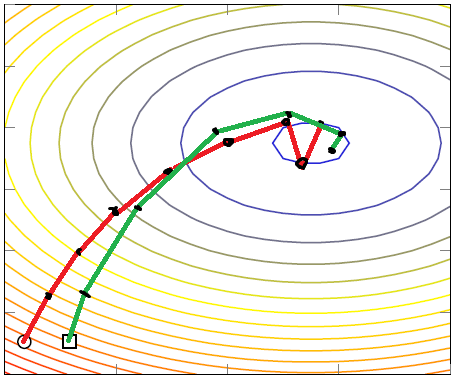
\includegraphics[width=0.95\textwidth]{./img/gradient.png}
\end{minipage}\begin{minipage}{0.6\textwidth}The normal gradient descent takes the gradient at the current position and then takes a step ($\propto$ learning rate) in this direction. This leads to unnecessary small steps when following a valley and too large steps at the end. GD with nesterov momentum first takes a step in direction of the momentum (approx. the same direction and length as the previous step) and then evaluates the gradient there and then takes a step with this ``lookahead''-gradient.
\end{minipage}
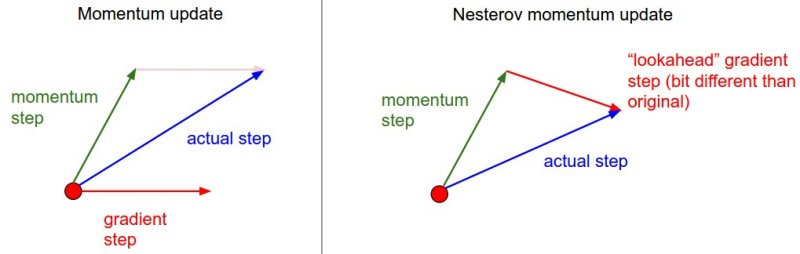
\includegraphics[width=\textwidth]{./img/nesterov.jpeg}
%
\section{Batch Gradient descent}
\subsection{Batch, minibatch, and stochastic gradient descent:}
The gradient descent algorithm starts at some point, looks for the direction of steepest descent and makes a step proportional to the learning rate in this direction to get to a (at least local) minimum (or critical point). Calculating this gradient on the whole dataset is computationally expensive, therefore usually only a subset of the training samples are used for each step. 

The following schemes exist\footnote{Source: \url{http://sebastianruder.com/optimizing-gradient-descent/index.html\#batchgradientdescent}}
\begin{itemize}
\item Stochastic gradient descent: Use only one sample --- the resulting path in the search space may be rather erratic
\item Batch gradient descent: Calculate gradient on the whole training data set. This is expensive and usually not necessary
\item Minibatch gradient descent: Middle path between SGD and BGD---calculate gradient on a subset of medium size (32 to 128 samples are used usually). The resulting behaviour is smoother than SGD and faster as BGD. 
\end{itemize}

Therefore MBGD is most commonly used.
%\subsection{Which version is most commonly used in deep learning and why?}
\subsection{What effects has the minibatch size?}
The size of the minibatch isn't a critical parameter. A bigger minibatch results in a smoother descent of the objective function but makes leaving local minima more difficult and is also computationally more expensive. 
\subsection{Pseudo-code of minibatch-based training and validation with early stopping}
\begin{lstlisting}
for each of 200 epochs:
    for each minibatch in training set:
        train classifier, store loss and training accuracy
    for each minibatch in validation set:
        test classifier, store validation accuracy
    compute and report means over loss and accuracies
    if accuracy is better then best model so far store model
    if accuracy did not improve in the last n (5-20) epochs restore best model and stop
\end{lstlisting}
%

\section{Weight and bias parameters}
\subsection{How do weight and bias parameters affect the input x?}
The weight parameter is applied multiplicative to x, and the bias is added. $w = Wx+b$
\subsection{What must be considered when initializing these parameters?}
The bias is less critical and can be set to $0$ for initializetion.

The weights are critical because of the multiplication and the gradient descent converges very different depending on the initialization. Extremely important is a difference in the weight matrix to break symmetry. A good  initialization is $Norm(0,1)\gamma$, the standard normal distribution times a hyper parameter $\gamma$ that controls the magnitude of the weights.
\subsection{What happens if the weights are set too large or too small?}
The hyper parameter $\gamma$ controls the magnitude of gradient and step size, so if set too large, the activation explodes, and if to small, the activation vanishes. In both cases, the algorithm most likely won't converge to a good model. 
\subsection{We discussed a heuristic for controlling the magnitude of weights. What is the intention behind this heuristic (no math required)?}
The so called Xavier initialization tries to set the weights in way to preserve the variance of the input which is usually $1$ with a mean of $0$ (due to normalization). When each neuron is connected to $D$ input neurons with weights sampled from $\gamma N(0,1)$ the resulting variance would be $\gamma^2 D\cdot 1$. Therefore $\gamma$ is set to $\gamma= 1/\sqrt{D}$ s.t. the variance of the result is $1$ again. 

He initialization is an adaption of this scheme with $\gamma = \sqrt{\nicefrac 2 D}$ that is optimized for ReLU activations.

\section{Preprocessing}
\subsection{Explain the purpose of preprocessing.}

The purpose is to cancel out variations that have a random cause(not related to class) thus should be neglected. For images, this are variations in brightness and contrast. Brightness can be normalized by mean subtraction. Contrast can be nromalized by division with standard deviation or by histogram equalization. The final image will have zero main and unit variance, which is the preferred input for ML settings.

\subsection{How do per-sample normalization and per-trainingset normalization differ in terms of operation and purpose?}

per sample normalization takes statistic for mean and variance over one image, while per trainingset normalization consider all images in the training set.

While per sample normalization has the benefit of cancelling out under/overexposed pictures or the ones with different contrast.

\todo{just a guess, not covered in lecture, can't find it in book}
Per sample normalization makes sure, that each sample has zero main and unit variance, but espacially for color image and per channel operation, this might yield in unwanted result (eg underwater picture will have almost 0 black channel, and this IS important).

Thus, per sample normalization should only be applied for all channels or B/W pictures.

\subsection{In the latter case, which (if any) preprocessing is applied during validation and testing?}

For the statistics, only the training set is used, but the normalization operations must be applied to the test and validation set.

\section{Optimization vs ML}
\subsection{What are the goals of optimization and machine learning?}

In optimization, the goal is to find optimal parameters that minimize the loss on the training set.  

For machine learning, we need an general model that works well on unseen data. 

\subsection{Why do they differ?}
A model with minimal loss on the training data is usualla an overfitting model that will not generalize well, and have worse results on unseen data. There are usually less specific parameters that have a higher loss on the training set, but work better on the test set.

\subsection{Create two sketches with each showing the training progress over time in terms of both training and test error; one that is good from an optimization perspective but bad from a machine learning perspective, and one that is worse from an optimization perspective but better from a machine learning perspective. Explain both sketches.}

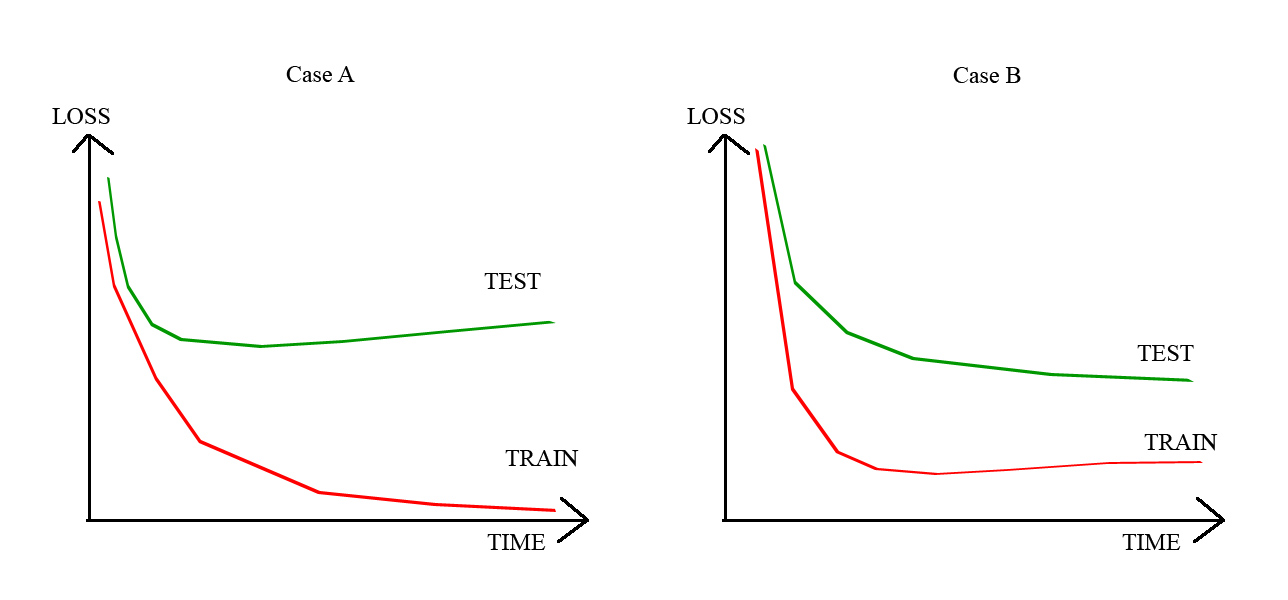
\includegraphics[width=\textwidth]{./img/optvsML.jpg}

Case A is the one with the focus on optimization, where the test set loss increases after w while, because the model overfits to the training data.

Case B is the desired outcome for ML, where we allow the training loss to stalls or even increases, as long as the test set loss decreases. This will yield a more general model as in Case A.

\section{Regularization}
\subsection{What is the purpose of regularization?}

As stated above, in ML we are interested in a low test error, not necessarely a low training error. Regularization is a method to achieve a better test error, but with a possible higher training error, by getting a more general model that has decreased model veriance (with increased biases) and is less prone to overfitting. 

\subsection{What is weight decay and what is its purpose?}
Weight decay is a common regulization technique, it penalizes too large weights (but leaves biases unaffected) which avoids that certain inputs have to much influence and allows the model to take all inputs into account. 

Weight must be initialized with 0 mean, and in each step, the weights are adjusted in a regulization step:

$L_{reg}(\Theta) = \frac{\delta}{2}||w||^2 + L(\Theta)$

where W is a vector of all weights and $\delta$ is the hyper parameter regulization strength(if too small: no effect, if too big: dominates data loss).
This way, all weights shrink in each update and decay to zero.  

\subsection{What is early stopping and how does it work?}
For early stopping a validation set is needed. It works on the observation, that when training overfitting-prone models, the training error will always decrease, while at some point the validation error will start to increase. 

So early stopping, a easy to implemnt and very common method, will store the model with the lowest validation error, and if the above situation occurs(no improvement or even higher error on validation after some iterations), stop and return the stored model.

\subsection{In deep learning, is it better to increase regularization or to decrease the model capacity by other means, and why?}
You should increase regulization, because in deep learning, models work best if they have enough capacity to overfit, but are regulized properly.

\section{Feedforward NN}
\subsection{What is the definition of a feedforward neural network?}
A FF NN does not have cycles (as a RNN for example has). The samples get passed to the input layer and the values are then passed forward until they reach the output layer where the result is evaluated.
\subsection{Which types of units do such networks have?}
\begin{minipage}{0.3\textwidth}
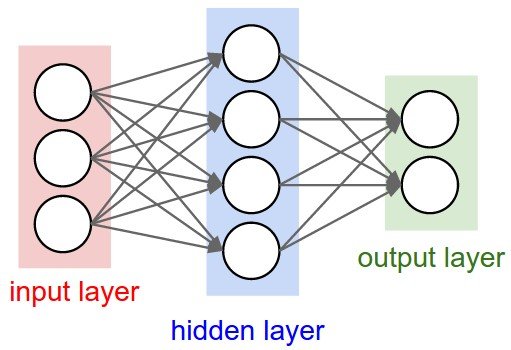
\includegraphics[width=\textwidth]{./img/ffnn1.jpeg}
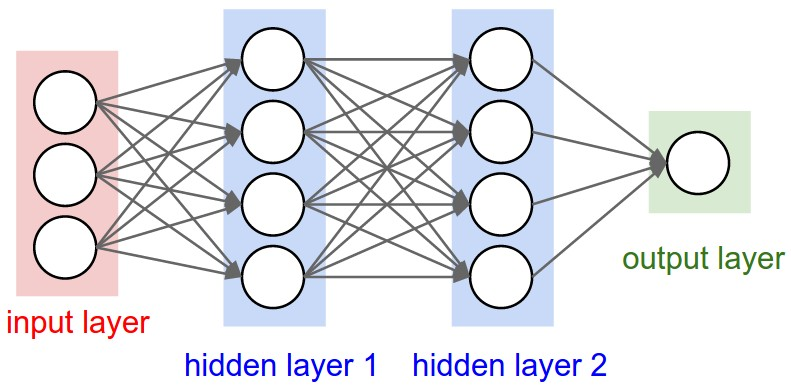
\includegraphics[width=\textwidth]{./img/ffnn2.jpeg}
\end{minipage}
\begin{minipage}{0.7\textwidth}
\begin{itemize}
\item Input units: Provide values, no computations, form the input layer
\item Hidden units: Are connected to previous layer (either input or a hidden layer) and calculate a linear combination of the inputs (sum of value of connected units times weight of connection) which is then passed through an activation function (identity for regression, ReLU or tanh for classification)
\item Output units: Last layer, may perform the same calculations as hidden layer.
\end{itemize}
\end{minipage}
%
\section{MLP}
\subsection{What is the definition of a multilayer perceptron?}
A MLP is a FF NN with input and output layer as well as some hidden layers. Neurons in layer $l$ are connected to all neurons in layer $l-1$ (dense/fully connected layers).
\subsection{What operation do (non-input) units perform?}
Each neuron at layer $l$ gets the output from the previous layer as input $x_l$ and calculates the input $x_{l+1}$ for the next layer by calculating $n_i(a_i^\top x_l + b_i)$ where $b_i$ is the bias, $n_i$ is the activation function and $a_i$ is the vector of weights of neuron $i$.
\subsection{What is an activation function and which functions are common?}
After calculating the linear combination $a_i^\top x_l$ (scalar product of input and weight vectors) the resulting value is passed to the input function. For regression the identity function is 	used whereas for classification task a nonlinear function such as $\mathrm{tanh}$ or ReLU ($\mathrm{max}(0,x)$ is used to enable nonlinearities.
\subsection{Why are multilayer perceptrons not suitable for deep learning for image analysis?}
MLP usually don't improve their performance with 3 or more layers. This makes it impossible to learn a hierarchy of features as DL does.
Also the number of parameters increases quickly with image dimensions.
%
\section{Representation learning}
\subsection{What is the motivation and purpose for representation learning?}
The idea behind representation learning is to extract features from images which are then used to train a model. Designing such features by hand is difficult though, therefore a two layer MLP approach is used: The first stage learns to extract features from the input and another stage then trains a linear classifier on these features.
\subsection{How is deep learning related to representation learning, and what is its definition?}
The problem with the outlined approach is that it must learn high level features in a single step. Deep learning is the idea to solve this problem in a divide and conquer way. 
Simple features that are easy to learn are combined to higher level features. The name DL is due to the many layers of this feature-hierarchy.
%
\section{Locally connected layers for image analysis}
\subsection{What is the motivation for using locally connected layers for image analysis? What is sparse connectivity}
An image consists of several features, some are local and some are global. In most cases, the global features are a combination of several local features in a certain arrangement.
The idea of locally connected layers is to train each layer only to extract features from some part of the image and then use additional layers to combine those. 

This is called sparse connectivity. Instead of connecting the $N$ input neurons with $N\times M$ connections (and corresponding weight) to the $M$ output neurons only connect each of the $M$ output neurons to some small subset of the input neurons. 
\subsection{Assume input data of dimension $W \times H \times D$. How many many weight and bias parameters does a locally connected (but not convolutional) layer have, assuming $3 \times 3$ connectivity and $W \times H \times 2$ output data dimension, and why?}
Every output neuron is connected to $9$ input neurons per channel, therefore $W\cdot H\cdot 2 \cdot 9 \cdot D$ weight parameters and $2$ bias parameters (one per feature map).\todo{not entirely sure that the number of bias params is correct}
%
\section{Convolutional Layer}
\subsection{What is the purpose of a convolutional layer?}
A convolutional layer is trained to extract features from the input. Early in the NN they aggregate information from input pixels in their receptive field (e.g. ``a stroke in this direction''). Deeper in the network such low level features are then combined again to form higher level features (``a stroke in this and in that direction'')\ldots.
They use spatial structure of the input by applying their filter kernel to a pixel and its neighbours. 
\subsection{How do such layers differ from locally connected layers, and why are they almost always preferred?}
Convolutional layers share their parameters, i.e. a kernel with a given size (often $3\times 3$) is applied starting from the top left and then moved in stepsizes corresponding to the stride. 
This differs from locally connected layers that don't share the parameters and have a set of weights for every output pixel.  As the features learned somewhere on the input are more often than not also useful on other parts of the input sharing the learned weights drastically reduces parameters while still maintaining accuracy.
\subsection{How many parameters does a convolutional layer have?}
A convolutional layer maps the $W \times H \times D$ input to $W' \times H' \times D'$ and has four hyperparameters:
\begin{itemize}
\item Number of filter $K$ -- this is then the output depth $D_o$
\item Spatial extent $F$
\item Stride $S$
\item Amount of zero padding $P$
\end{itemize}
and must learn a $F\times F$ kernel for each of the $K$ filter and each of the $D$ input layers as well as a bias parameter for every layer in the output, therefore $F\cdot  F\cdot  D' \cdot  D$ weight parameters and $K$ bias parameters. 
\subsection{What are feature maps?}
A feature map is obtained by applying a filter to the input. This is done by dragging the kernel in stepsizes corresponding to the stride over the input and calculate a new value for every step. The resulting filter map size depends on stride and zero padding as well as the size of the input: $W' = (W-F+2P)/S +1$ (same for height).
%
\section{Receptive field}
\subsection{What is the receptive field of a neuron?}
The receptive field is the region of the input that is seen by a certain neuron (directly or indirectly connected).
\subsection{Assume a network consisting of two convolutional layers with $3 \times 3$ connectivity followed by a $2 \times 2$ max-pooling with stride 2 and again two convolutional layers with $3 \times 3$ connectivity. What is the receptive field of neurons in the final convolutional layer? How does the receptive field affect feature extraction? }
Each $3\times 3$ conv. Layer increases the receptive field by two neurons. A pooling layer with stride two increases the receptive field by a factor of 2. Starting from the final layer we have:
\begin{align*}
\text{Receptive field increase} = (1+2+2) \cdot 2 + 2+ 2 = 14
\end{align*}
This is the increase in one dimension, therefore the receptive field of one final neuron is an area of $14\times 14$ neurons (input pixels).
A neuron can only extract a feature if it is in the receptive field. Therefore the higher level features in the final layers of the NN should have a receptive field that spans the whole (or at least almost the whole) input.
\subsection{Why do convolutional layers usually use $3 \times 3$ connectivity?}
As the number of parameters depends with $O(n^2)$ on the filter size a stack of 3 $3\times 3$ layer has approximately as much weights to learn as a single $5\times 5$ layer. Therefore more smaller filters are usually preferred as additional layers improve the modelling of nonlinearity.
%
\section{Pooling}
\subsection{What is the purpose of pooling layers?}
Reduce spatial size to reduce amount of parameters and computation. Also helps against overfitting. Consolidate features learned in convolutional layers before the pooling layer.
\subsection{Calculate the output of a 2 × 2 max-pooling layer with stride 2 assuming the following input.}
\begin{equation}
pool\left(\begin{bmatrix}
1 & 1 & 2 & 4\\
5&6&7&8\\
3&2&1&0\\
1&2&3&4
\end{bmatrix}\right) = \begin{bmatrix}6 & 8 \\3 & 4\end{bmatrix}
\end{equation}
\subsection{How many pooling layers with stride 2 should a CNN have assuming an input resolution of 64 × 64 and convolutional layers that do not change the resolution, and why?}
The highest level features should have a receptive field that spans more or less the entire image. 4 to 5 pooling layers should therefore be a good choice. Exact number may vary based on the overall architecture.
\todo{How many pooling layers should CNN have?}
%
\section{CNN}
\subsection{Give a general overview of convolutional neural networks and their purpose}
A convolutional neural network is a NN that consists of an input layer and several convolutional layers with many filters. Often convolutional layers are mixed with pooling layers to reduce the input size and the amount of parameters to learn. 

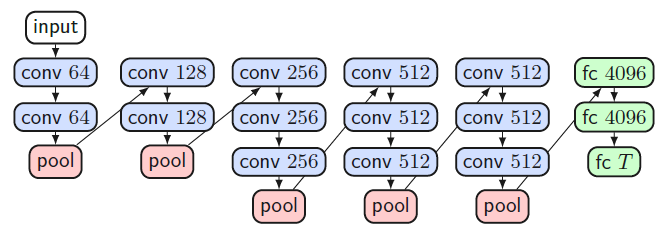
\includegraphics[width=\textwidth]{./img/cnn.png}
\subsection{What are the two overall stages of such networks?}
\begin{itemize}
\item Frontend: Consists of convolutional and pooling layers and is used to extract features
\item Backend: Usually consists of one or two dense (fc) layers and is used to combine features learned in previous layers to make class predictions. 
\end{itemize}
\subsection{How is the depth of a CNN defined?}
Depth is defined as the number of layers with parameters to learn and is thus mainly determined by the number of convolutional layers.
\subsection{What effect does increasing the depth have?}
A higher depth allows higher levels of abstraction. At least $6$ conv layers should be used according to slides. Networks with higher depth may result in better performance, though with diminishing returns. In the case of ResNet the performance gains obtained by going from depth 50 to 100 is approx. twice as large as from going from 100 to 200. Without ResNet like architecture training more than 30 layers may be difficult though (increasing layers on VGGNet from 20 to 50 increases error rate as optimization algorithm doesn't find good parameters any more).
\subsection{How does one choose a suitable network depth to solve a given image classification problem?}
Current state of the art networks use many layers that learn features that achieve linear separability which allows simpler backends consisting of only one dense layer. When choosing higher depths additional measures must be used to still be able to efficiently train the model:
\begin{itemize}
\item Better initialization algorithms: Prevents signal from exploding or vanishing. Necessary that model with 30 ReLU layers even converges
\item Batch normalization: Normalize output of layers to zero mean and std 1. Means and scaling factors are learned during training and should then be applied in testing mode. 
\item Residual learning: Propagte input to output before computing activation function. If optimal mapping is closer to identity small fluctuations are easier to find
\end{itemize}
\todo{how to choose network depth for image classification problem}
%
\section{CNN backends}
\subsection{What is the backend of a CNN?}
In the backend the features extracted by the frontend are used to classify the samples. The last layer is therefore usually a dense (fc) layer with neuron count corresponding to the number of classes. 
\subsection{Discuss the backends of VGGNet and GoogLeNet/ResNet and their pros and cons.}
\begin{itemize}
\item VGGNet: Uses two fc 4096 layers followed by a fc $T$ ($T= \text{number of classes}$).  Many parameters due to this MLP with two large hidden layers (later research revealed that these could be omitted with no performance downgrade)
\item GoogLeNet: Average (instead of max as usual) pooling layer over the whole width and height of the previous layer, reducing the dimension from $W\times H\times D$ to $D$ (number of filters of previous layer). These $D$ features are then mapped to the classes with a single fc layer.
\item ResNet: Same backend as GoogLeNet
\end{itemize}
%
\section{ResNets}
\url{http://kaiminghe.com/icml16tutorial/icml2016_tutorial_deep_residual_networks_kaiminghe.pdf}
\subsection{What are residual networks (ResNets) and which problem do they overcome?}
\begin{minipage}{0.4\textwidth}
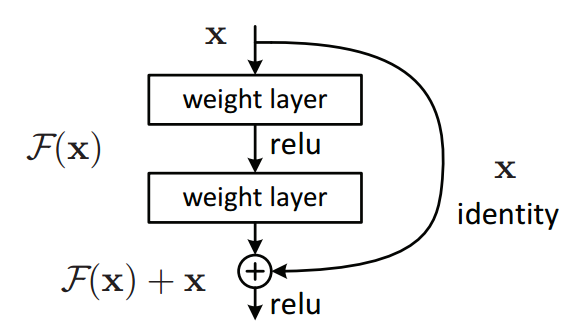
\includegraphics[width=\textwidth]{./img/residual.png}
\end{minipage}
\begin{minipage}{0.6\textwidth}
ResNets are the current state of the art architecture. They consist of residual blocks which are composed of two $3\times 3$ conv layers. An additional additive residual function $\mathcal F$ is learned that decides what should be added or removed from the input. 
\end{minipage}

The output from a layer is added to all subsequent layers instead of propagated by multiplication with the weights from deeper layers. This makes the partial derivations also additive and prevents vanishing of the signal during backpropagation and enables efficient learning of nets with higher depth. 
%
\section{Back Propagation}
\subsection{What is the purpose of the backpropagation algorithm?}
\begin{itemize}
\item { Compute gradient of computation graph given by NN and current parameters}
\item { Starting from input calculate derivatives of all nodes by their children. Sum up derivatives multiplied over all paths from output to input node to get derivation of output by input node. }
\item { Gets inefficient really fast if multiple paths from input to output exist. Reverse accumulation strategies help in this case (reverse mode differentation)}
\end{itemize}
\subsection{Example}
\tikzset{
  treenode/.style = {align=center, inner sep=0pt, text centered,font=\sffamily},
  calc/.style = {treenode, circle, draw=black, black,fill=green!25, text width=1.5em},
  numbr/.style = {treenode, circle, draw=black, black,fill=red!25, text width=1.5em},
  input/.style = {treenode, circle, draw=black, black,fill=blue!25, text width=1.5em},
}
\begin{minipage}{0.6\textwidth}
\begin{tikzpicture}[->,>=stealth',level/.style={sibling distance = 5cm/#1,
  level distance = 1.5cm}] 
\node [calc] {* 455}
    child{ node [calc] {+ 35} 
            child{ node [numbr] {5}  edge from parent node[above left]{$1$}}
            child{ node [calc] {* 30 } 
		child{ node [input] {5}edge from parent node[left]{$5$}}
		child{ node [input] {6} coordinate (AA) edge from parent node[right]{$6$}}
		edge from parent node[above right]{$1$}
            }            edge from parent node[above]{$13$}                
    }
            	child{ node [calc] {+ 13}   coordinate (BB)
			child{ node [input] {7}edge from parent node[below right]{$1$}}
			edge from parent node[right]{$35$}
	            }    
; 
\draw[->,>=stealth']( $ (BB)!15pt!(AA) $ )--( $ (AA)!10pt!(BB) $ );
\end{tikzpicture}
\end{minipage}\begin{minipage}{0.4\textwidth}
\begin{align*}
\partial a &= 13\cdot 1 \cdot 5 = 65\\
\partial b &=  13\cdot 1 \cdot 6 + 35\cdot 1 = 113\\
\partial c &= 35 \cdot 1 = 35
\end{align*}
\end{minipage}
\subsection{Explain the steps of the algorithm at a given node.}
\begin{itemize}
\item { First calculate values at every node}
\item{ Then derive each node by input parameters to get partial derivatives}
\item{ Multiply every path from an input to output (chain rule $g(f)' = g'(f)\cdot f'$}
\item { Sum up all paths from input to output (product rule: $(g\cdot f)' = g'\cdot f + f'\cdot g$}
\end{itemize}
%
\section{Data Augmentation}
\subsection{What is the purpose of data augmentation?}
The bigger the training set the better the resulting NN can be. As obtaining huge datasets is not easy a good approach to circumvent this is extending the dataset at hand by various transformations such as mirroring, changing lighting, rotations, affine transformations, croppping, \ldots
\subsection{What transformations work /don't work for a digit classifier}
\begin{itemize}
\item Everything related to color/lighting does more or less not apply here as digits may be written by a pen of any color and therefore transforming the b/w should be the best approach
\item Mirroring does not work on either axis
\item Rotating the samples is a good idea as people may have a different skew in their writing. Though the rotation angle should be in a range between $\pm 10-20^\circ$. Using arbitrary rotations is a bad idea as e.g. a ``6'' would then be mixed up with a ``9''.
\end{itemize}
%
\section{Dropout}
\todo{dropout section is rather weak}
\subsection{What is the purpose of dropout, how does it work, and why is it effective?}
\begin{minipage}{0.4\textwidth}
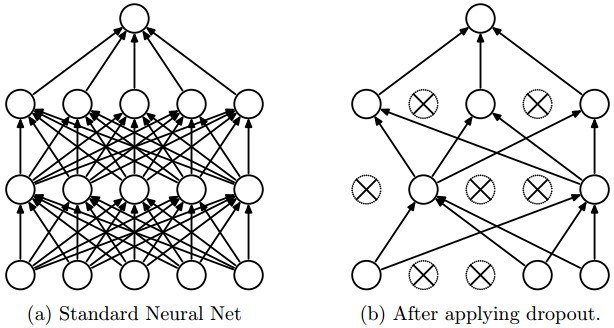
\includegraphics[width=\textwidth]{./img/dropout.jpeg}
\end{minipage}
\begin{minipage}{0.6\textwidth}
Dropout sets the output of a neuron to 0 with probability $p$ during training. This temporarily discards certain neurons which helps with regularization because the net tries to prevent depending too much on certain features. 
\end{minipage}
\subsection{Why do ``dropped'' neurons have no effect on the output of the next layer?}
The outputs are scaled with the dropout probability to prevent an effect from the dropout.\todo{this is almost certainly wrong}
\subsection{To which CNN layers is dropout commonly applied?}
GoogLeNet applies dropout to the final pooling layer. ResNet does not use dropout. 
\todo{where to apply dropout?}
%
%: Batch normalization
%
\section{Learning rate}
\subsection{What does the learning rate hyperparameter specify?}
The direction of steepest decrease can be calculated with the gradient, the size of the optimal stepsize is unknown and instead the stepsize given by the learning rate hyperparameter is used. The choice of this parameter is critical. 

If learning rate is:
\begin{itemize}
\item very high: Gradient descent algorithm jumps over minima and is more or less a random walk in configuration space
\item high: Finds a better configuration then the random starting configuration but gets stuck there as it ``oscillates'' around minimum (e.g. minimum is in a circle with radius 2 and algorithm makes steps with size 5
\end{itemize}
\begin{minipage}{0.6\textwidth}
\begin{itemize}
\item proper: First missclassification rate quickly decreases and then slowly converges to some minimum
\item low: Finds minimum as well but very slow (progress looks linear whereas in the beginning almost exponential decay of error should be possible)
\end{itemize}
\end{minipage}\begin{minipage}{0.4\textwidth}
\hspace{0.2cm}\includegraphics[width=\textwidth]{./img/learningRates.jpeg}
\end{minipage}
\subsection{Explain a heuristic for adapting the learning rate during training and why doing so can be beneficial.}
Learning rate decay can be used to tune the learning rate to the optimal choice at each step. First start with a rather high learning rate and when there is no improvement for a few epochs scale the learning rate with a constant factor (e.g. $\nicefrac 1 2$).
Alternatively scale the learning rate every 5-20 epochs with a factor ($\nicefrac 1 2$ to $\nicefrac 1 {10}$). This ensures that big steps are taken by the algorithm when it is possible but the stepsize is reduced when further improvements can only be made by smaller steps.
%
\section{Oversampling}
\subsection{What is the purpose of oversampling and how does it work?}
A sampled passed to the neural net may depict something know but the viewpoint may be slightly off or the lighting may be unusual. Oversampling tries to overcome this challenge by applying various transformations to the image, classifying all transformed versions separately and average the class scores of the results. 
\subsection{What is ten-crop oversampling?}
Ten-crop oversampling is a common technique which consists of making five crops of the image, one in the center and in all four corners and then using the 5 resulting images as well as their mirrored versions for classification. 
\subsection{What transformation could be applied for dog breed classification.}
\begin{itemize}
\item Ten-crop oversampling
\item Mirroring
\item Rotation
\item Skewing images
\item Adapting brightness
\end{itemize}
%
\section{Model ensembles}
\subsection{What is the purpose and intuition behind using model ensembles?}
As a CNN is trained starting from a random initialization different models may perform well on different samples. Model ensembles try to exploit this by taking a set of models (at most 10 models) that are trained independently and let each of the models classify the sample and then average over their predictions.
\subsection{How might the individual models differ from each other?}
\begin{itemize}
\item Various architectures
\item Employing different data augmentation techniques
\item Different initial weights
\end{itemize}
%
\section{Medical tasks}
\subsection{What are the challenges in using medical imaging data?}
\begin{itemize}
\item Small datasets/study populations
\item Heterogenity of pathology
\item Treatment response
\item Subject specific variances
\item Developmental differences
\item Annotation needs experts
\end{itemize}
\subsection{Can deep networks be used effectively for medical tasks (give 3 examples)?}
\todo{Describe medical applications for CNNs}
\begin{itemize}
\item Pathology detection: Images of possible pathogens, 2D/2.5D/3D, Using CNNs. Input are e.g. images from MRT and network is used to assist diagnosis
\item Segmentation:
\item Shape modelling: Vessel detection in images with deep CNNs
\item Classification: 
\item Action recognition: Use RNNs to recognize surgical activities from robot kinematics
\end{itemize}
\subsection{How can we use the training data most efficiently?}
\todo{Medical appl.: How can we use the training data most efficiently?}
Train traditional CNN with negative and positive samples. Use the false positives as extra instances for training the fine-tuned CNN.
\subsection{Give an explanation of the methodologies fine tuning and transfer learning and the benefit using them in medical imaging. }
\begin{itemize}
\item Transfer learning: Train a CNN on huge dataset (ImageNet) and use the intermediate feature layers (up to the FC layer which connects to the 1000 classes) as feature extractor for the medical dataset. 
\item Fine-tuning: This method extends transfer learning. The idea is to retrain some of the deeper layers trained on ImageNet with the medical dataset as many features may be relevant for certain classes that are not present in the medical domain. It is usually a good idea to use different learning rates for the untrained and the pretrained layers.
\end{itemize}

%
\section{2-3D deep CNN}
\todo{Maybe provide additional information here}
\subsection{What is the difference between 2D, 2.5D and 3D deep CNN networks?}
\begin{itemize}
\item 2D: Takes image as input (X-Ray)
\item 2.5D: Takes 3 images from orthogonal directions (3 X-Rays)
\item 3D: Take many images, for example with MRT. Then either take Z 2 dimensional kernels or one three dimensional kernel.
\end{itemize}

%: CNNs in medical imaging
\section{Labelling}
\todo{Non-expert annotation information is very sparse in slides}
\subsection{Explain the challenges, benefits and drawbacks of using expert vs. non-experts to obtain labels of medical image data?}
\begin{itemize}
\item Expert labelling:
\begin{itemize}
\item Expensive
\item Time consuming
\item Publicly availabe ground truth data may not be available
\end{itemize}
\item Non-expert labelling
\begin{itemize}
\item Annotations from single non-experts noisy
\item Disagreements
\item Crowd of non-experts can perform as well as medical experts
\end{itemize}
\end{itemize}
\subsection{Give  an example of an alternative method to expert-based manual labeling of medical data for deep learning approaches.}
Crowdsourcing labels: Instead of using experts for annotation use a crowd of non experts. Add additional layer that aggregates the input from the crowd.

Example: Agg-Net (Deep Learning From Crowds for Mitosis Detection) had an aggregation layer, using CNN to weigh the votes of the different users with varying precision. The result are of the same quality as the ones from experts.
%
\section{RNNs}
\subsection{Describe the main purpose of RNNs and give an example application.}
RNNs are suited for temporal machine learning task, where not a single instance has to be taken into account, but a number of instances where the order is importent. One example would be text generation, where the task is to create a single character or word, but the previous characters/words are very important for the next item. Video analysis, e.g. classification would be another example, where the isn't just a single image, but a whole video stream of several frames.
\subsection{Draw and explain a sketch illustrating the overall  architecture of such networks.}
\begin{minipage}{0.3\textwidth}
\hspace*{1cm}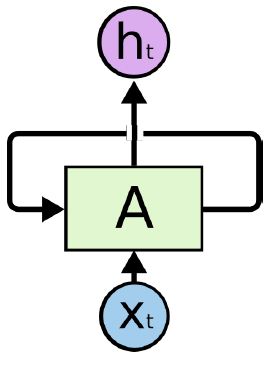
\includegraphics[width=0.6\textwidth]{./img/rnn.png}
\end{minipage}
\begin{minipage}{0.7\textwidth}
The main feature of RNNS are loops sucht that information can be passed from one temporal step to the next. Thus, the next state of A does not only depend on input $x_t$, for the step $t$, but also on the previous state of $A_{t-1}$. $h_t$ is the output of the network at step $t$.
\end{minipage}
\subsection{What is the main limitation of traditional RNNs (as opposed to LSTMs)?}
A problem arises, when the important information is not only one or at least a few (defined) steps before t, but when it could be from an arbitrarily far away step. In the given example ``I grew up in Italy ... I speak fluent \textit{italian}'' the important word to inference the language is Italy.  The larger the potential gap, the more complicated the problem becomes. 
%
\section{LSTMs}
\subsection{What is the main advantage of LSTMs over traditional RNNs?}
LSTMs are designed for rememembering informations for long periods of time. So they solve above mentioned problem
\subsection{Draw a sketch that illustrates the dataflow within a LSTM block.}
\begin{minipage}{\textwidth}
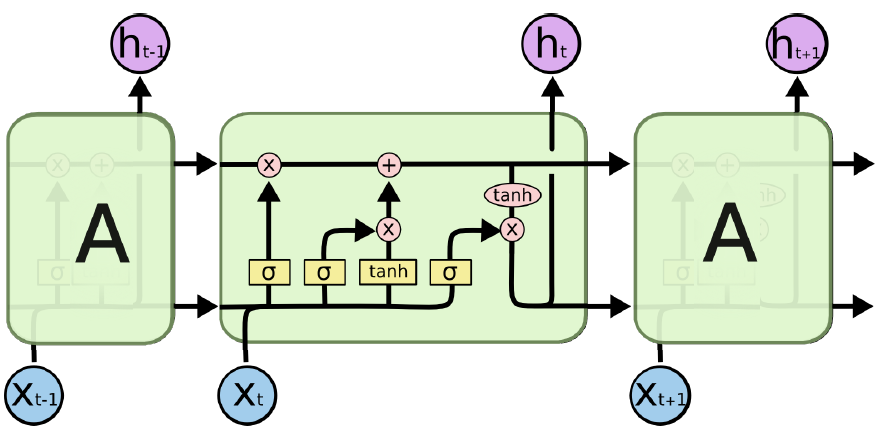
\includegraphics[width=\textwidth]{./img/lstm.png}
\end{minipage}
The Cell state C, the upper line, contains the core information. It is controlled by several
sigmoid gates. 
\subsection{List and explain the purpose of the different LSTM gates.}
The left gate is the forget layer, which takes information from the previous output and the current input to get a multiplicative value between 0 and 1 for each information in C.

The middle gate is the input layer. It decides which values to update and create new candidate values for C.

The right gate is the output gate, which takes the updated and filtered state C, the previous output and the input to create a new output.

\addtocounter{section}{-1}\section{}\label{sec:done}